\section{Bilag}
\subsection{Test}
\subsubsection{Test a dice}\label{diceTest}
\begin{lstlisting}[language=Java, caption=Dice is random test]
import static org.junit.jupiter.api.Assertions.*;

public class DiceTest {
    

    /** Test af JUnit for at teste at det er sat korrekt op.
     * Her testes der blot om der er en konstruktør i Dice klassen */
    @org.junit.Test
    public void constructorExists() {
        Dice d1 = new Dice();
        assertEquals(Dice.class, d1.getClass());
    }


    /** diceIsRandom testen skal teste hvorledes metoden roll() i klassen Dice er tilfældig,
     * når den skal slå et tal fra 1-6 */
    @org.junit.Test
    public void diceIsRandom() {
        int diceRoll;
        int diceCount = 0;

        Dice d1 = new Dice();

        for (int i = 0; i < 100000; i++) {
            diceRoll = d1.roll();
            //Det antages at med 1 terning vil vi ca. få hvert slag 16.666 gange ud af
            //de 100.000 slag.
            if(diceRoll == 1) {
                diceCount++;
            }
        }

        //Vi tester om terningen slår 1. 16.666 gange, med 1% afvigelse
        if (diceCount < 16500 || diceCount > 16832) {
            fail("Terningen er ikke tilfældig, da den slog 1. færre eller flere gange end forventet");
        }
    }
}
\end{lstlisting}

\subsubsection{Test a ChanceKort}\label{ChanceKortTest}
\begin{lstlisting}[language=Java, caption=ChanceKort is random test]
import java.lang.reflect.Method;

import static org.junit.jupiter.api.Assertions.*;

public class ChanceKortTest {

    
    //Testen her er lavet på alle 24 kort, derfor fejler den nu, hvor der kun er 10 kort. Testen var en succes, da der var 24 kort. Dette ses også i rapporten.
    @org.junit.Test
    public void ChanceKortIsRandom() {
        int kort;
        int kortCounter = 0;

        ChanceKort kortTest = new ChanceKort();

        for (int i = 0; i < 1000000; i++) {
            kort = kortTest.randomChanceKort();

            //Det antages at ud af 24 kort er chancen for at trække kort 1. = 1/24
            //
            // Hvis vi trækker et kort 1.000.000 gange, bør vi få kort 1.
            // ca. 41.666 gange.
            if (kort == 1) {
                kortCounter++;
            }
        }
        System.out.println(kortCounter);
        //Nu tester vi om vi har trukket kort 1 det forventede antal gange
        //Vi tager hensyn til afvigelser, så vi tester med 1% afvigelse fra det forventede antal
        if (kortCounter < 41250 || kortCounter > 42082){
            fail("Du trak ikke kort 1. det forventede antal gange. Metoden er altså ikke tilfældig");
        }
    }

    @org.junit.Test
    public void RunChanceKortHas10Cards() throws ClassNotFoundException {
        //Expected er 12. 10 kort + 2 ekstra metoder, til at fjerne og tilføje biler.
        int expected = 12;
        int actual = 0;
        Class c = Class.forName("RunChanceKort");
        Method methods[] = c.getDeclaredMethods();
        for (int i = 0; i < methods.length; i++) {
            actual++;
        }
        assertEquals(expected, actual);
    }
}
\end{lstlisting}

\subsection{Gruppekontrakt}
\begin{figure}[H]
    \centering
    
\includegraphics[width=17cm]{figures/Gruppekontrakt1.jpg}
\end{figure}
\begin{figure}[H]
    \centering
    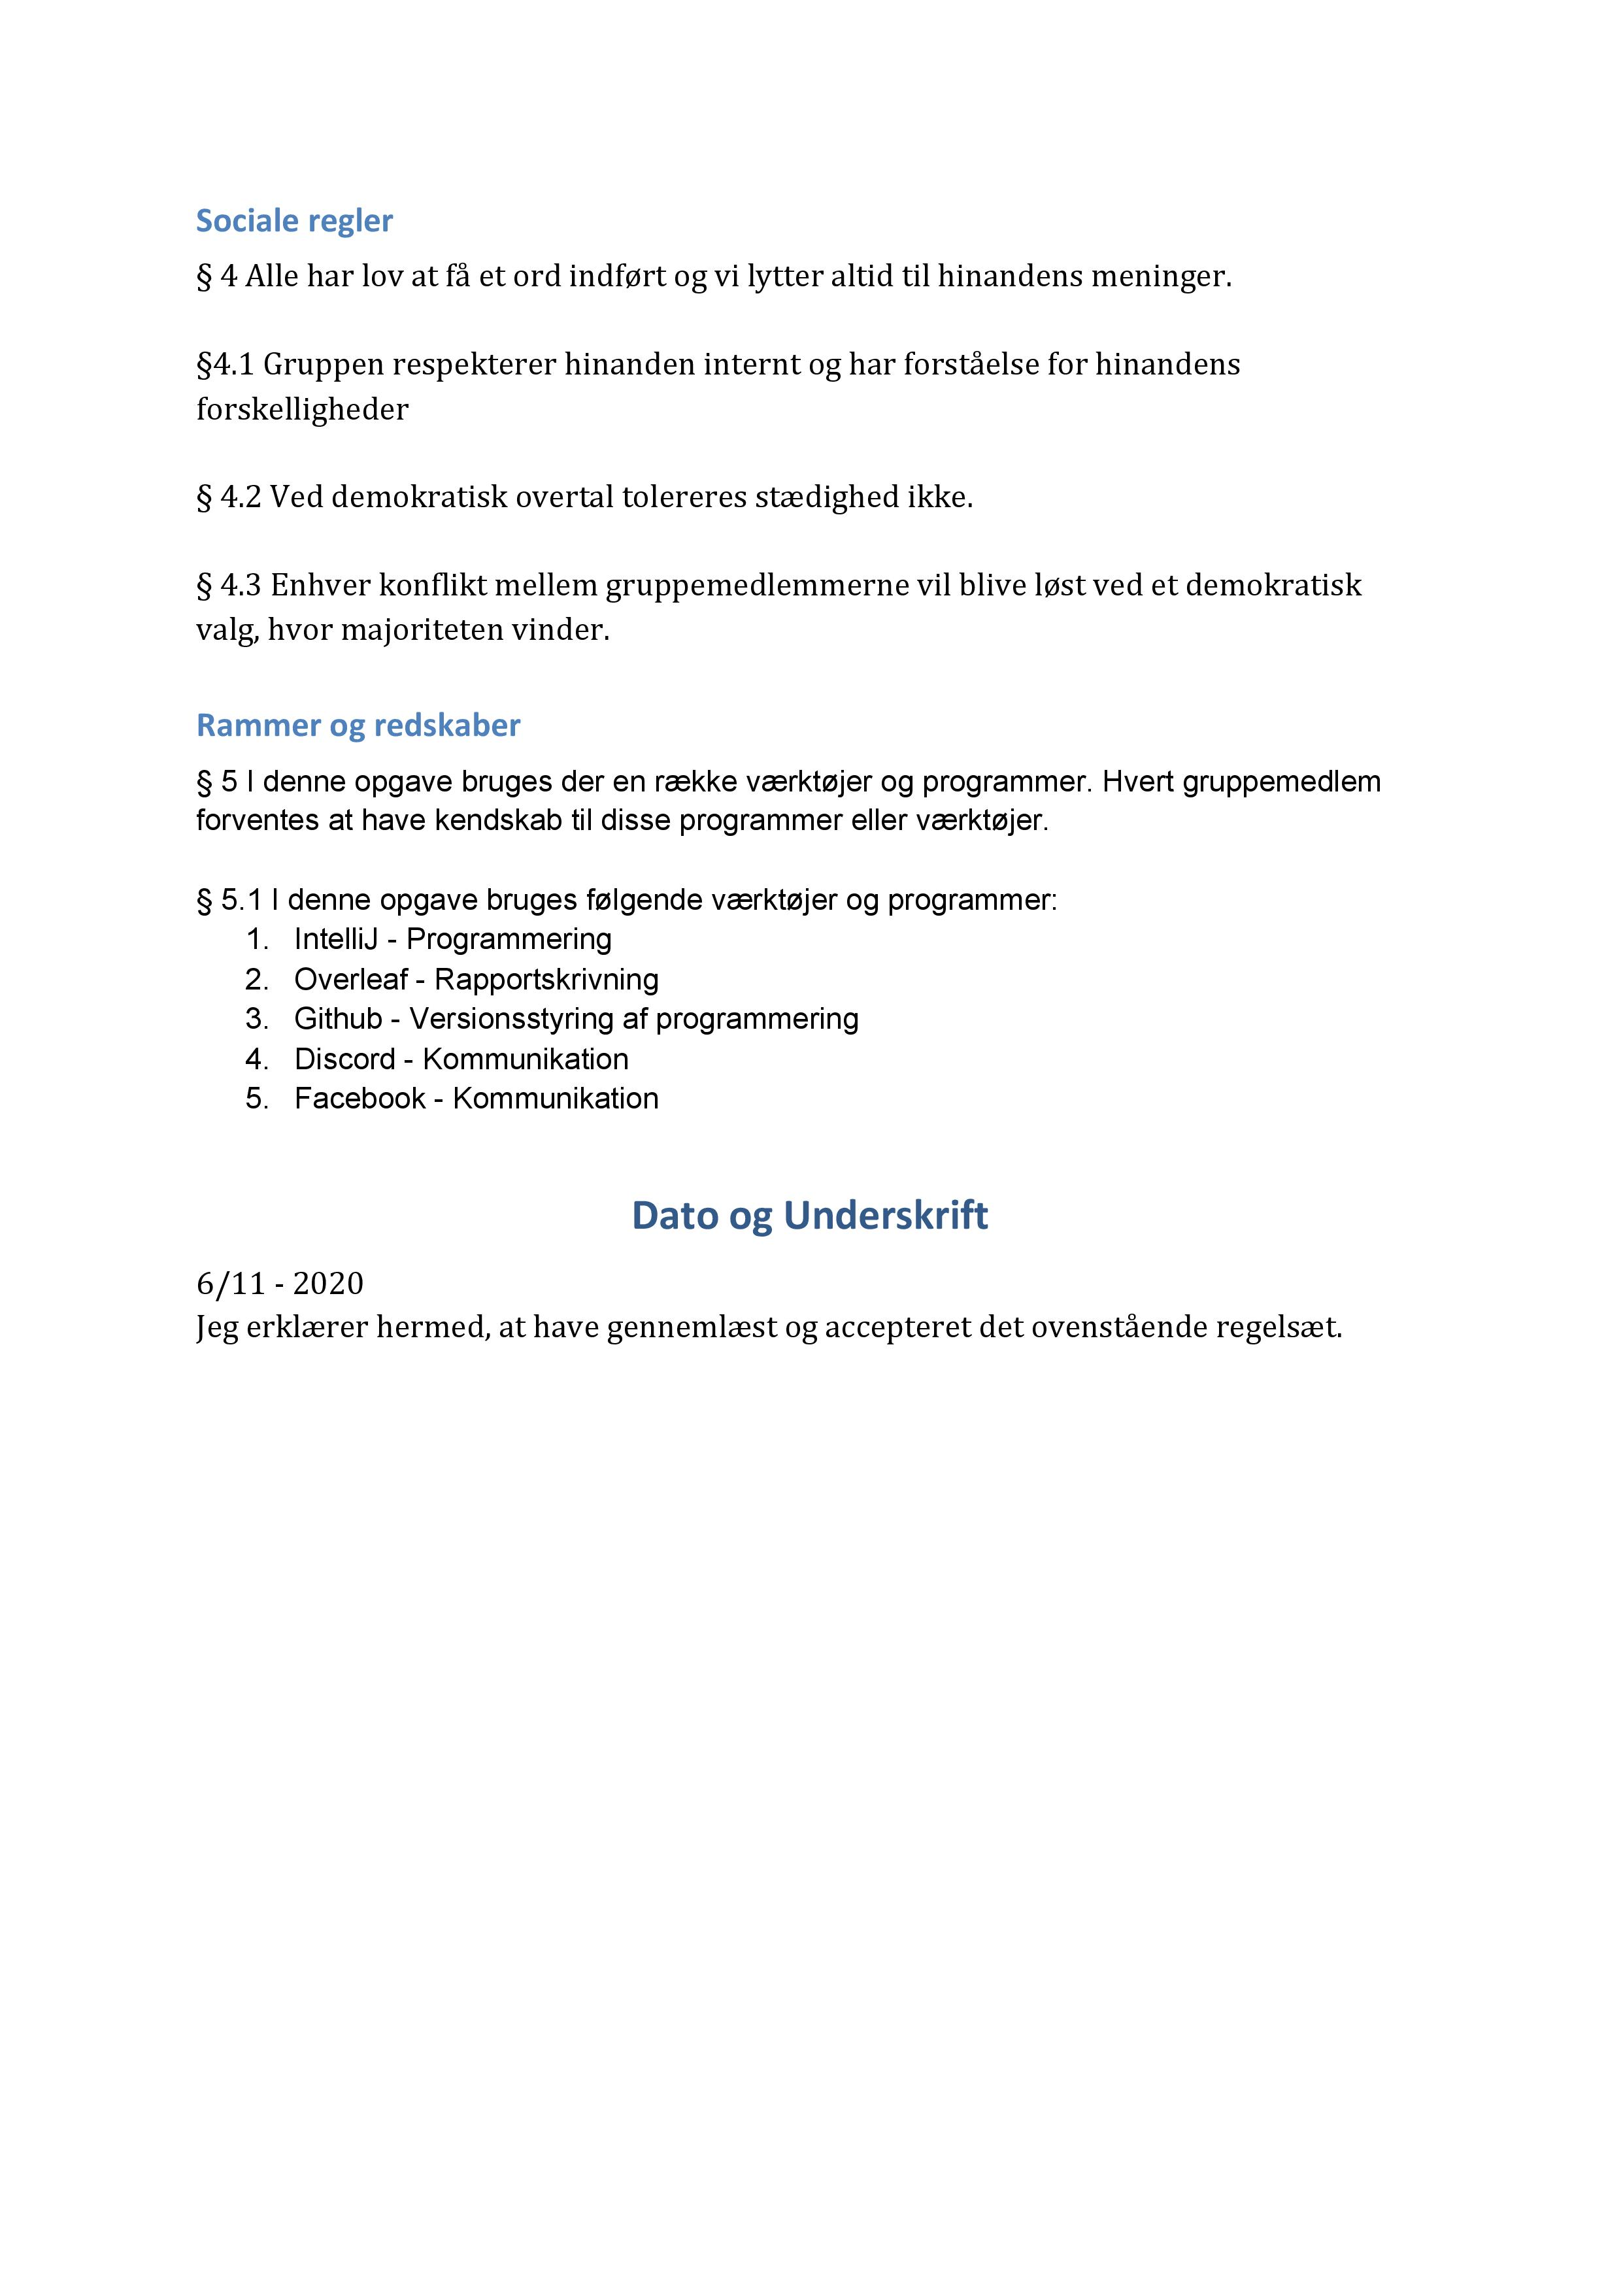
\includegraphics[width=17cm]{figures/Gruppekontrakt2.jpg}
\end{figure}